\documentclass[a4j,11pt,uplatex,twocolumn]{article}

\usepackage[dvipdfmx]{graphicx}
\usepackage[dvipdfmx]{color}
% \usepackage{url}
% \usepackage[top=30truemm,bottom=30truemm,left=25truemm,right=25truemm]{geometry}

\title{First Impression on \\``Asynchronous Consensus-Free Transaction Systems"}
\author{Shoma Mori}
\date{\today}

\begin{document}

\maketitle

\section{Motivation}
In existing blockchain systems, it is assumed that the consensus problem needs to be solved.
Payment transacton systems, which are one of the dominant ways to utilize blockchain, are also required to get a consensus in order to avoid double-spending problems.
However, making a consensus on transactions takes time, thus preventing scalability.
Therefore, blockchain could get scalability if systems can be managed without making a consensus, and they would be used more in practice.

In fact, if some node makes transactions whose sending addresses are the same using the same UTXO (Unspent Transaction Output), it is technically easy to find that behavior (Fig.~\ref{fig:double-spending}).
\begin{figure}[tbp]
    \begin{center}
        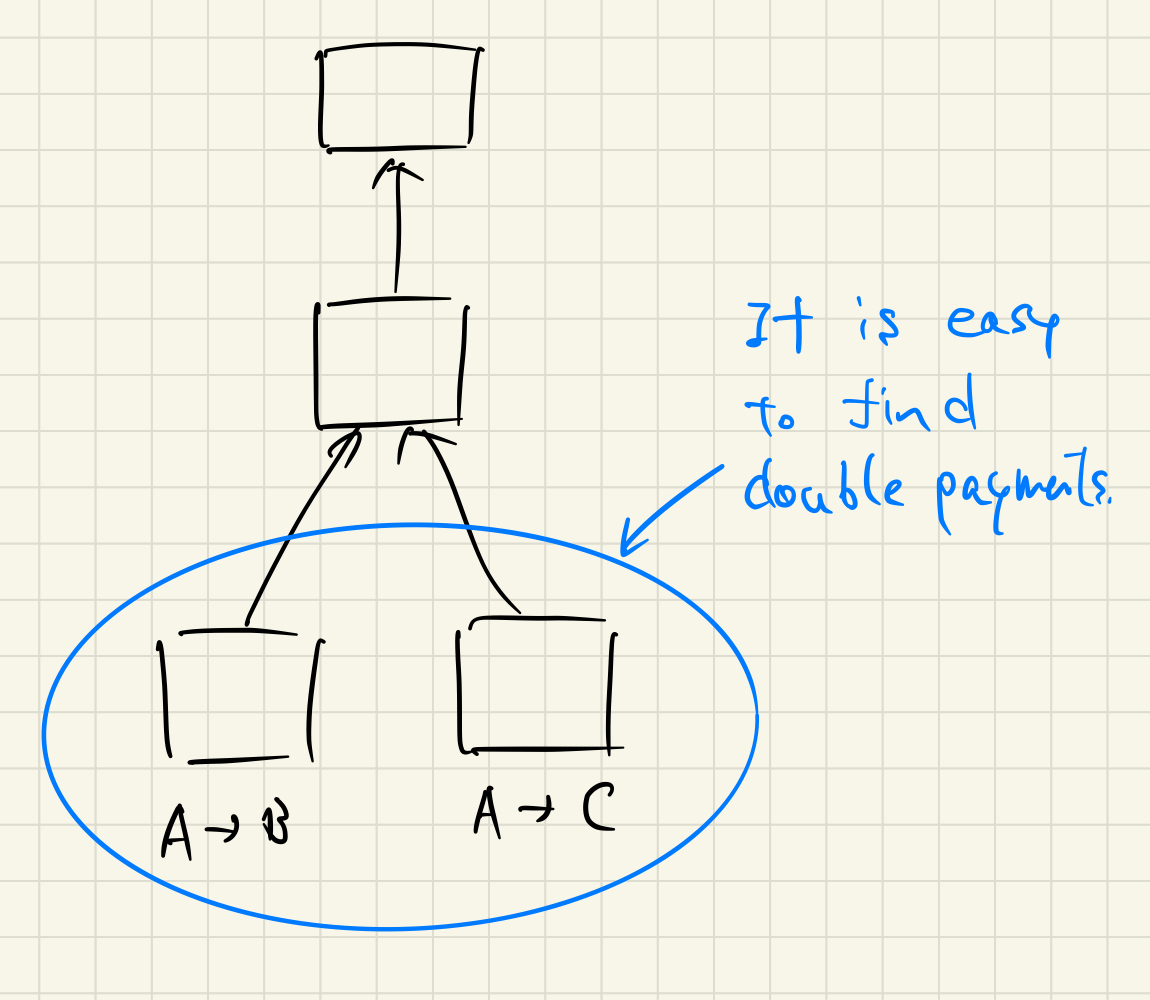
\includegraphics[width=6.0cm]{./fig/double_payments.jpeg}
        \caption{Double-spending}
        \label{fig:double-spending}
    \end{center}
\end{figure}
Moreover, it is obvious for the sender that he/she made a double payment since they actually paid.
Therefore, if systems have ``validators", who verify transactions, they do not need a consensus on transactions in terms of solving double-spending problems.

\section{Transactions\&Blocks}
The following is the flow that describes how a transaction from node $v_1$ to node $v_2$ is added to blockchain in our systems without a consensus.

\begin{enumerate}
    \item $v_1$ makes a transaction whose transfer destination is $v_2$'address using one UTXO linked to $v_1$'s address.
    \item $v_1$ broadcasts the transaction to its neighbors.
    \item Every node including validators receives the transaction.
    \item Validators verify whether the UTXO that is used as input in the transaction has not used yet by tracing blockchain.
    \item If not, validators include the transaction in their creating blocks.
    \item Validators broadcast their own new blocks when enough transactions are added to the blocks.
    \item Each node who received new blocks verifies whether every transaction in the blocks is valid by tracing blockchain as well.
    \item If all the transactions are valid, nodes add the blocks to their (local) blockchains.
\end{enumerate}

Nodes may want to add transactions whose UTXOs for inputs are already used, i.e. double-spending.
In order to resolve this problem, the systems deny transactions whose inputs are the same as a transaction in blockchain but their outputs are different.
Since transactions are broadcasted to the system, every node eventually gets the set of transactions and can detect the incorrect situation (Fig.~\ref{fig:conflict}).
When such transactions are detected, it is required to reject all the transactions which are related to the double payment because if one of them is made remained in blockchain, the system needs a consensus to choose the one.
\begin{figure}[tbp]
    \begin{center}
        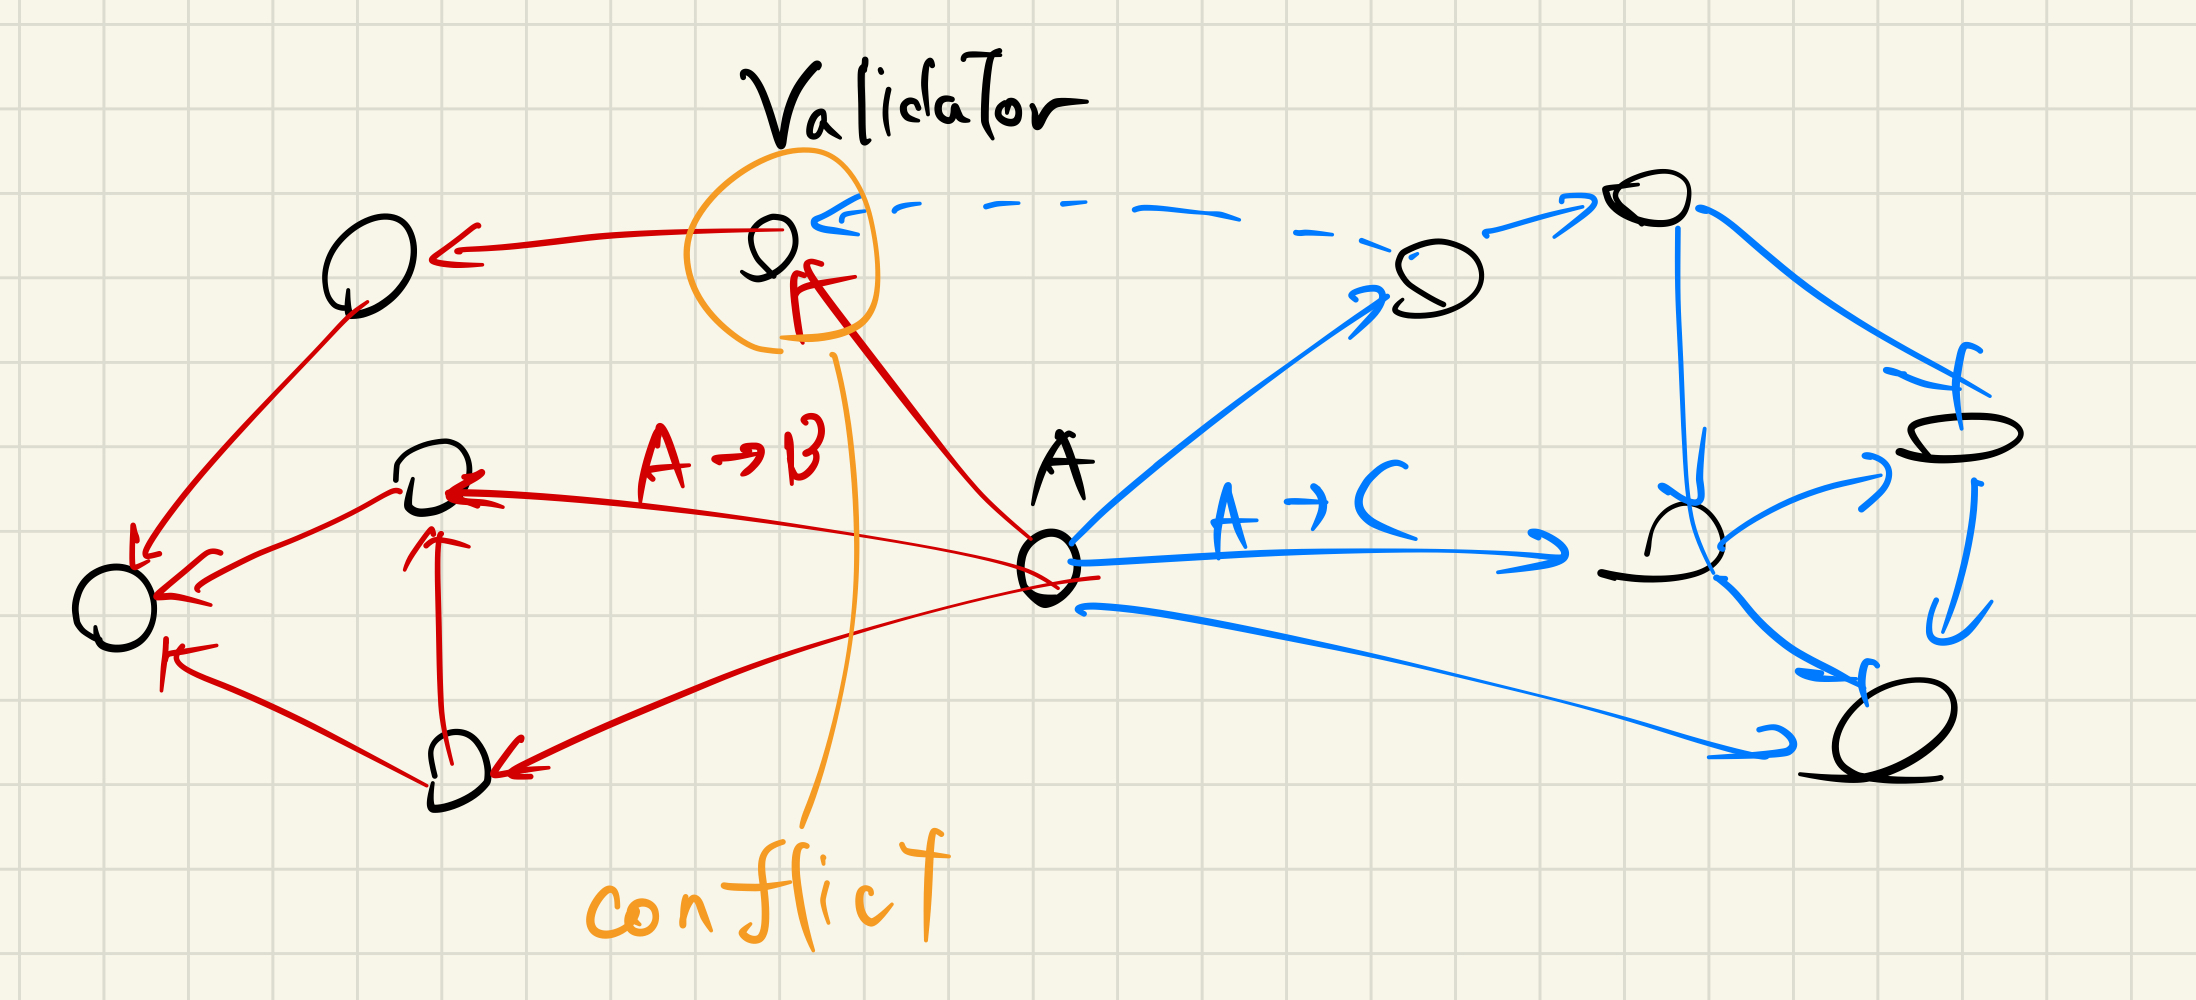
\includegraphics[width=8.0cm]{./fig/conflict.jpeg}
        \caption{Node A tries to make a double payment (A$\rightarrow$B and A$\rightarrow$C), but a validator detects a conflict by tracing blockchain.}
        \label{fig:conflict}
    \end{center}
\end{figure}

There is a possibility that nodes receive blocks whose parents are the same node.
Since the system does not make a consensus, it is not possible to choose leaders that connect to each parent.
In other words, blockchain can fork, that is, it is possible that the same transaction can be included in different blocks and the blocks can be added to blockchain.
Fig.~\ref{fig:different-blocks} shows the case where two different blocks which include the same transaction are created and broadcasted to the network.
In that case, the system can merge the two blocks into one block (Fig.~\ref{fig:merge}).
\begin{figure}[tbp]
    \begin{center}
        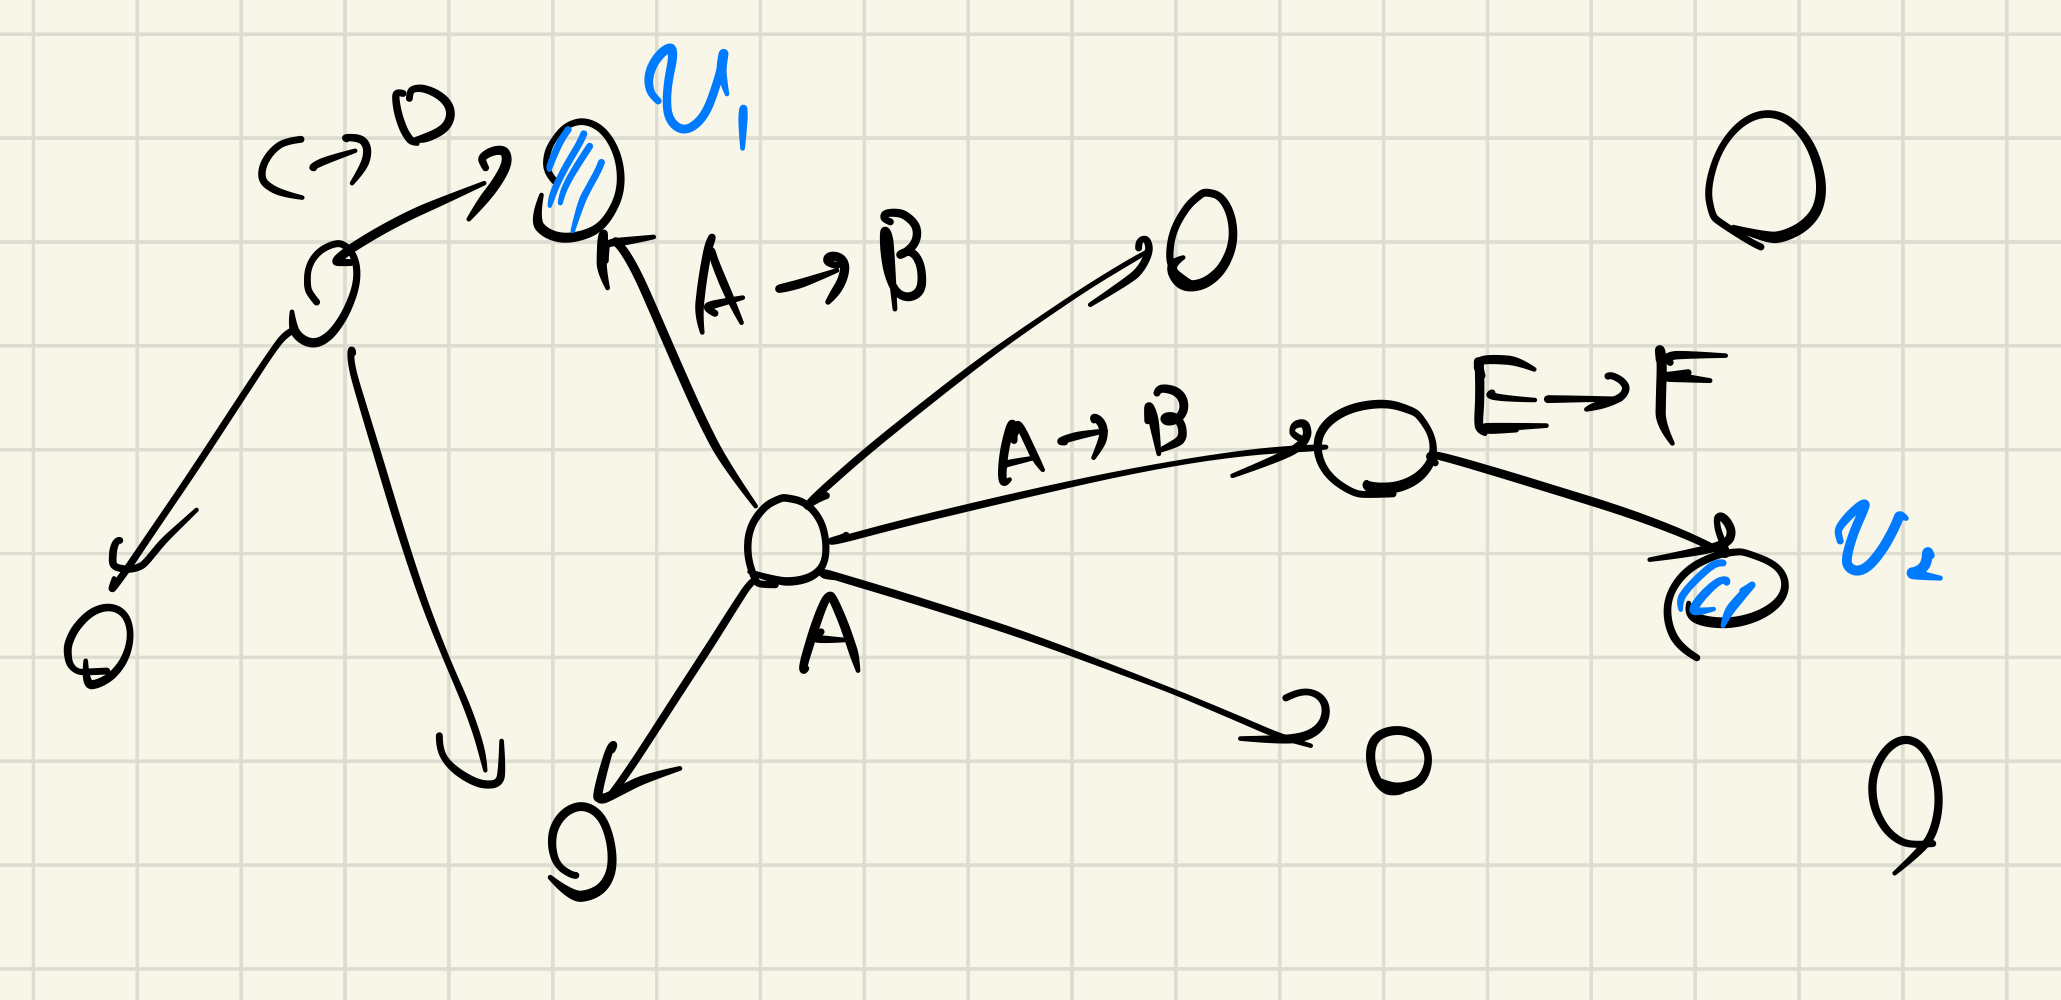
\includegraphics[width=8.0cm]{./fig/different-blocks.jpeg}
        \caption{Two different blocks which include the same transaction (A$\rightarrow$B) may be created because of the difference of the delivery order of transactions.}
        \label{fig:different-blocks}
    \end{center}
\end{figure}

\begin{figure}[tbp]
    \begin{center}
        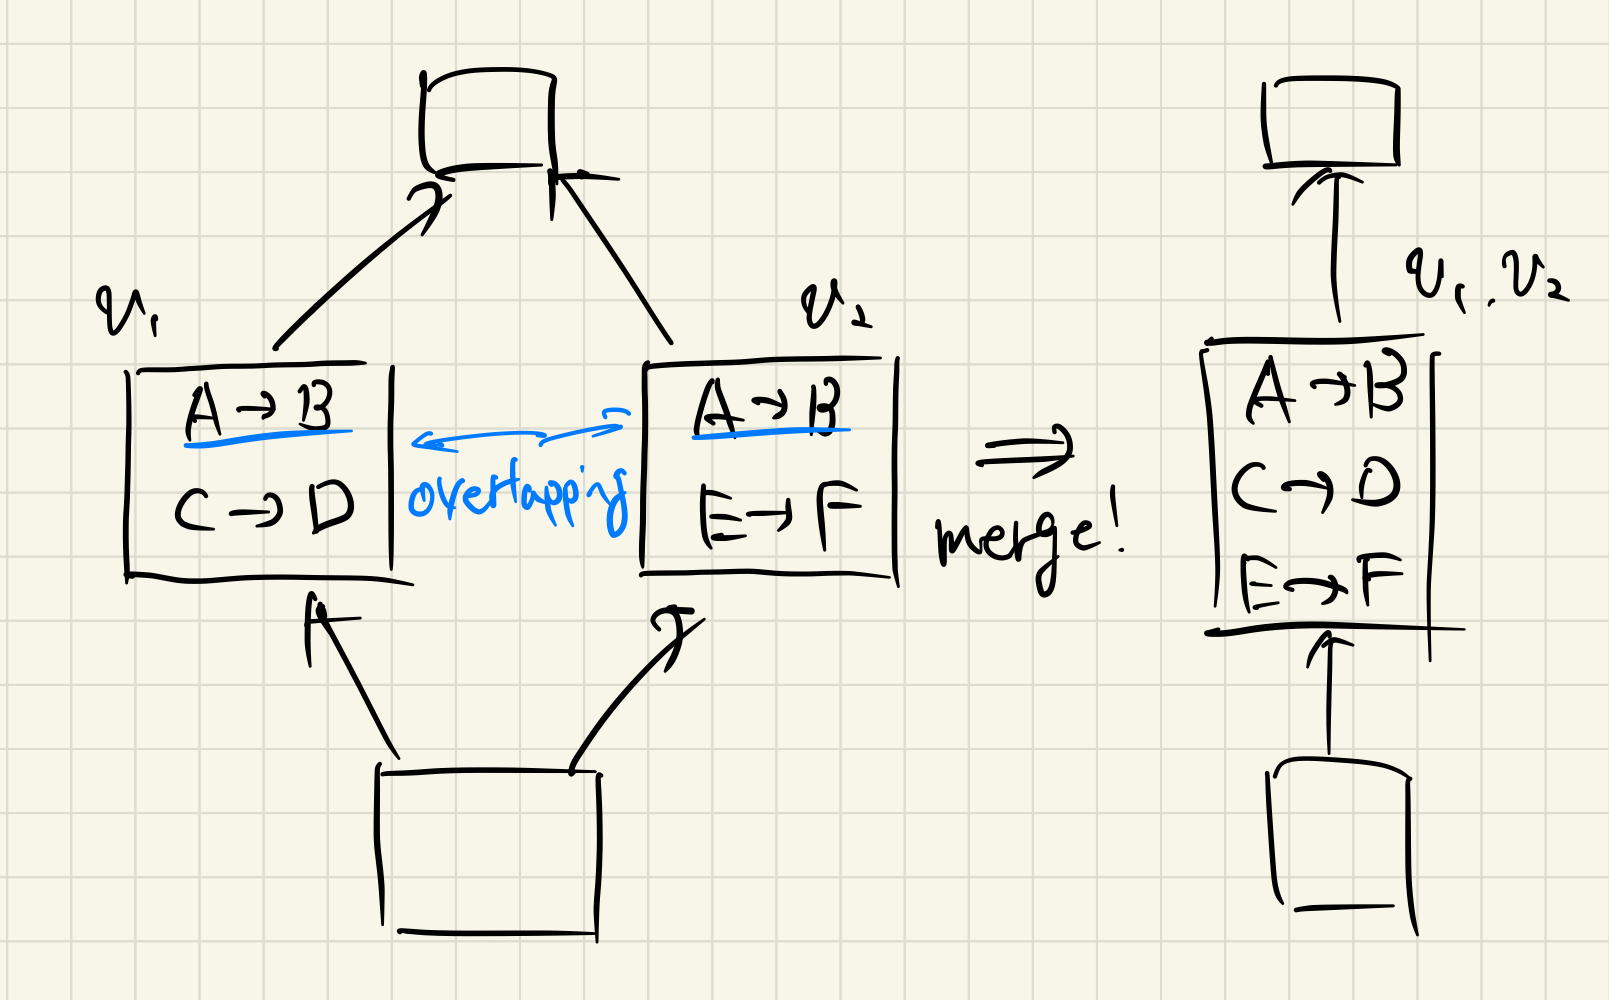
\includegraphics[width=8.0cm]{./fig/merge.jpeg}
        \caption{Blocks which have the same transactions can be merged into one block.}
        \label{fig:merge}
    \end{center}
\end{figure}

It is also possible that only some nodes are merged and other nodes are not.
This case can happen when a node receives a block whose parent is the same as the merged block.
In this case, if the other nodes are also merged into one block again, it may need to recalculate the child, perhaps even grandchild and so on because child node may be added to the merged node.
\begin{figure}[tbp]
    \begin{center}
        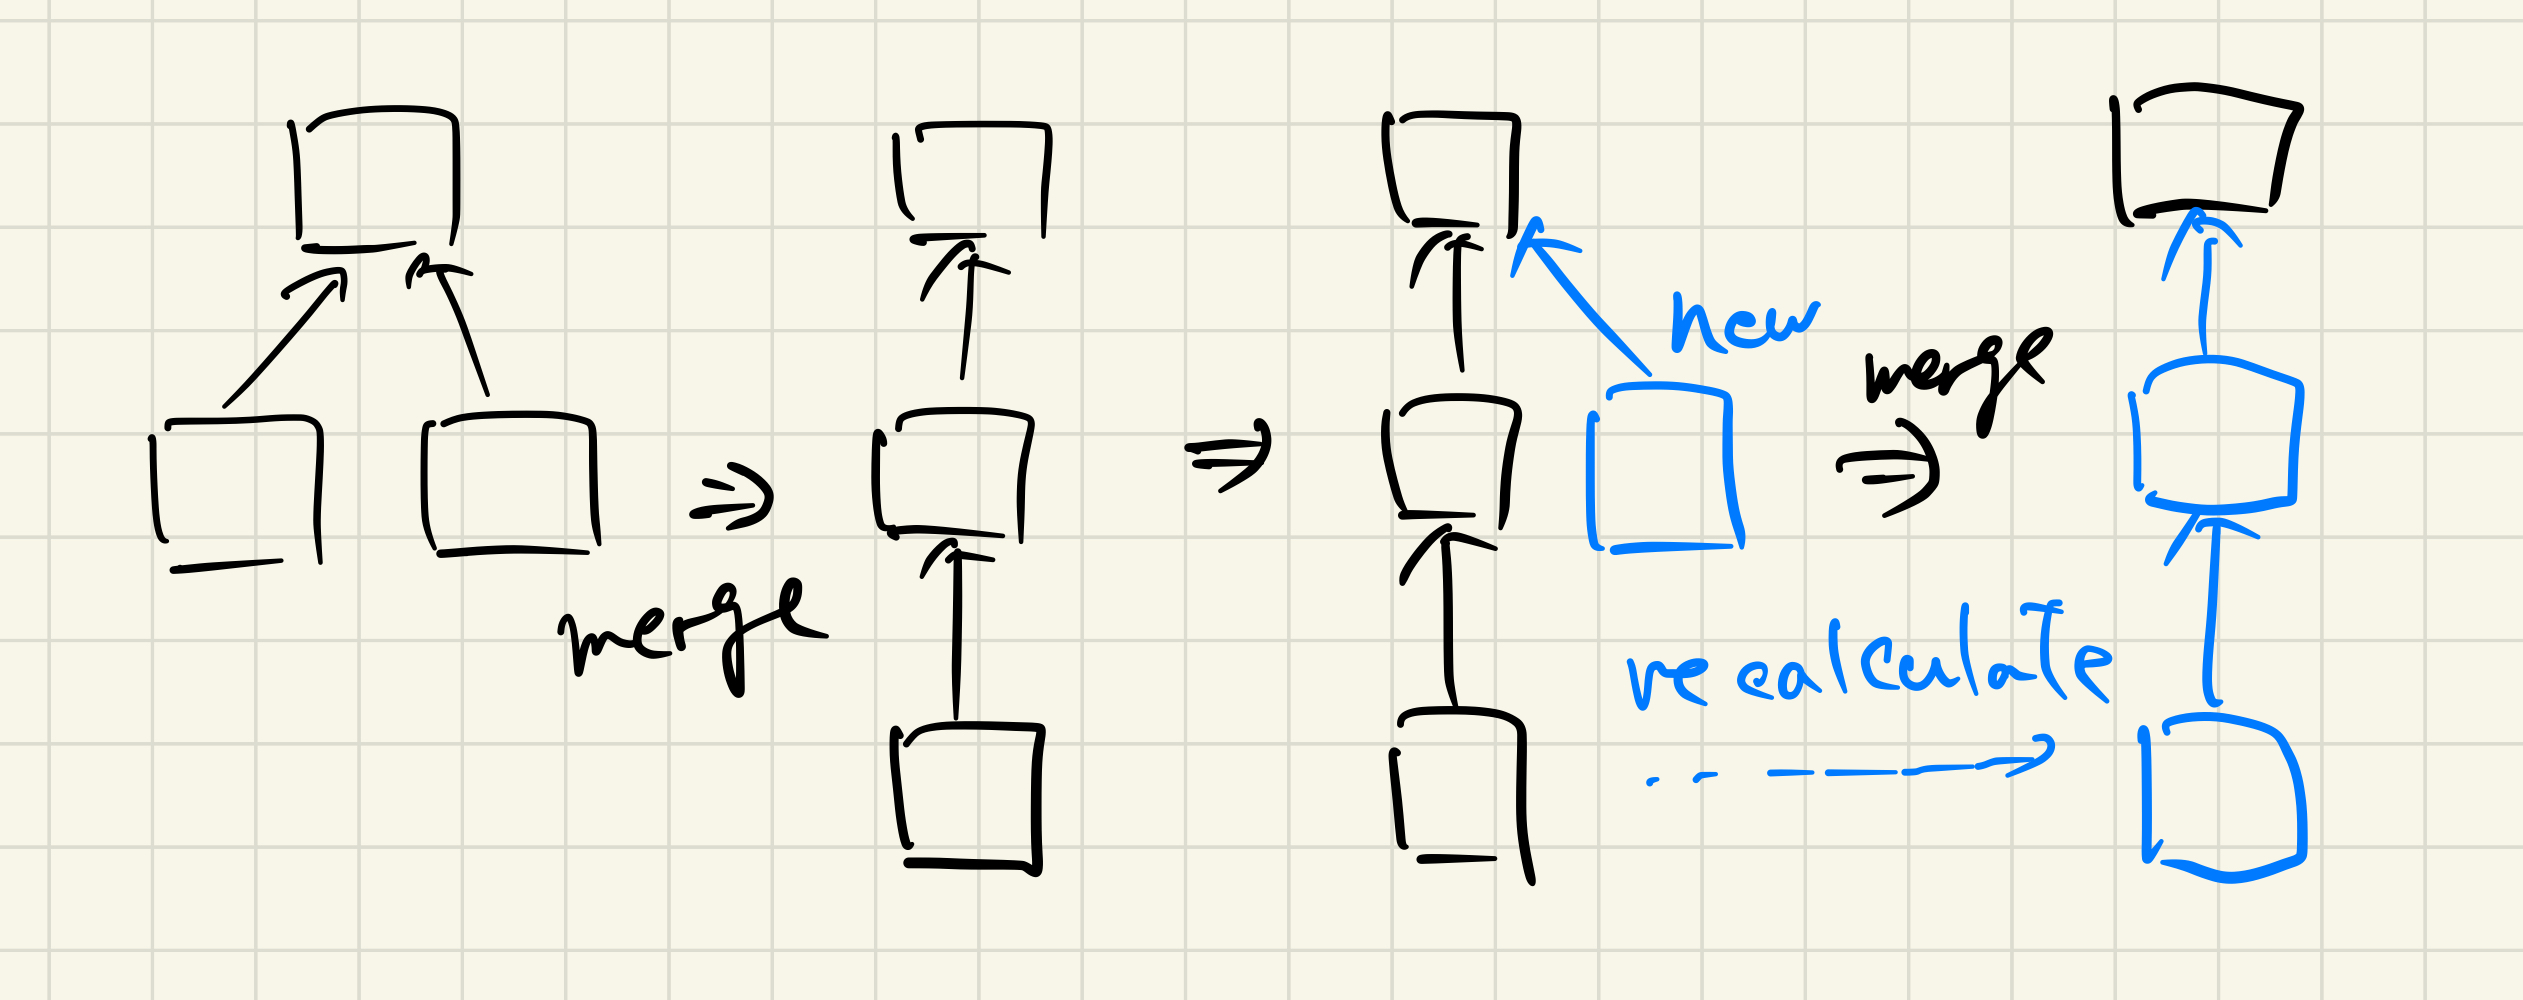
\includegraphics[width=7.5cm]{./fig/recalculate.jpeg}
        \caption{The case where a node received a block whose parent is the same as the merged block. If the system remerges the new block to merged block, its descendant must be recalculated.}
        \label{fig:recalculate}
    \end{center}
\end{figure}

\section{Open Questions}
In our systems, blocks can be added to blockchain without any workload or voting, which is different from blockchain systems with consensus algorithms.
Therefore, every node can make forks in order to try to tamper the history of transactions.
However, it can be avoided by rejecting double-spending transactions as described before.
The question is why we need to use blochchain.
I mean, we can also use an ordinary database to record transactions.

On the other hand, blockchain systems adopting PoW, for example, are not tampered easily since if someone tries to tamper some block, he/she has to tamper all blocks after the block, which needs tremendous workload.
That is why the shape of ``chain" is meaningful.

In our systems, however, since nothing is required to add blocks, it seems that recording in blockchain is essentially the same as recording in ordinary databases, such as RDB.
What is the advantage of using blockchain in our systems?
Or, in the first place, we do not assume to use blockchain?


























\end{document}


